\chapter{Еще одно исследование управляемости}
\label{ch:chap2}
\section{Условие задачи}

Продолжаем рассматривать систему:
$$
  \dot{x} = Ax + Bu
$$ и выполнить следующие шаги:

\begin{itemize}
    \item Проверить обе точки $x_1', x_1''$ на принадлежность управляемому подпространству
    системы. Принять целевой точкой x1 ту, что принадлежит.
    \item Выполните все шаги Задания 1 для рассматриваемой системы и выбранной целевой точки x1.
\end{itemize}

\section{Решение задачи}

Параметры для объекта:
$$
  A = \begin{bmatrix}
    3   &	-6	&  4 \\
    4   &   -5  &  4 \\
    -4  &    4  &  -5
  \end{bmatrix} \tab
  B = \begin{bmatrix}
    11 \\ 7 \\ -7 
  \end{bmatrix} \tab
  x_1' = \begin{bmatrix}
    1 \\ 0 \\ 0 
  \end{bmatrix} \tab
  x_1'' = \begin{bmatrix}
  0 \\ 0 \\ 1
  \end{bmatrix} 
$$

\subsection{Принадлежность точек управляемому подпространству}


Проверим принадлежность точек, для этого должно выполниться следующие условие для точки $x$:
$$
    rank(U) = rank([U x])
$$
Для начала найдём матрицу управляемости(склейка):
$$
    U = \begin{bmatrix}
        B & AB & A^2B
    \end{bmatrix} = \begin{bmatrix}
                    11   &	-37	&  79 \\
                    7   &   -19  &  23 \\
                    -7  &    19  &  -23
                \end{bmatrix}
$$
В нашем случае, для $x_1'$:
$$
rank(\begin{bmatrix}
    11   &	-37	&  79 \\
    7   &   -19  &  23 \\
    -7  &    19  &  -23
\end{bmatrix}) = rank(\begin{bmatrix}
    11   &	-37	&  79   & 1\\
    7   &   -19  &  23  & 0\\
    -7  &    19  &  -23 & 0
\end{bmatrix})
$$
$$2 = 2$$
Нетрудно заметить, что в обеих сторонах равенства будет по одно паре линейно зависимых строк. 
Значит точка $x_1'$ принадлежит управляемому подпространству.
В нашем случае, для $x_1'$:
$$
rank(\begin{bmatrix}
    11   &	-37	&  79 \\
    7   &   -19  &  23 \\
    -7  &    19  &  -23
\end{bmatrix}) = rank(\begin{bmatrix}
    11   &	-37	&  79   & 0\\
    7   &   -19  &  23  & 0\\
    -7  &    19  &  -23 & 1
\end{bmatrix})
$$
$$2 = 3$$
Ранги не равны, а значит точка $x_1''$ не будет принадлежать управляемому подпространству.

В итоге, $\mathbf{x_1' = x_1}$, идём дальше и выполняем все проверки из задания 1.

\subsection{Исследование управляемости системы}

$$
U = \begin{bmatrix}
    B & AB & A^2B
\end{bmatrix} = \begin{bmatrix}
                11   &	-37	&  79 \\
                7   &   -19  &  23 \\
                -7  &    19  &  -23
            \end{bmatrix}
$$
$$
  rank(U) = 2
$$
По критерию Калмана, наша система не полностью управляема по состоянию, так как ранк матрицы управляемости не равен порядку системы.

Найдём собственные числа матрицы $A$:
$$
    \lambda_{1,2} = -3 \pm 2i, \tab \lambda_3 = -1 
$$

Вычислим матрицу Хаутуса для каждого собственного числа:
$$
    H_1 = \begin{bmatrix}
          A - \lambda_1 I & B   
          \end{bmatrix} = 
    \begin{bmatrix}
    6-2i & -6 & 4 & 11 \\  
    4 & -2-2i & 4 & 7 \\  
    -4 & 4 & -2 -2i & -7   
    \end{bmatrix}
$$
$$
rank(H_1) = 3
$$
Значит собственное число $\lambda_1$ является управляемым, если ранг его матрицы Хаутуса равняется порядку системы.
$$
    H_2 = \begin{bmatrix}
          A - \lambda_2 I & B   
          \end{bmatrix} = 
    \begin{bmatrix}
      6+2i & -6 & 4 & 11 \\  
      4 & -2+2i & 4 & 7 \\  
      -4 & 4 & -2+2i & -7  
    \end{bmatrix}
$$
$$
rank(H_2) = 3
$$
Аналогично, собственное число $\lambda_2$ является управляемым.
$$
    H_3 = \begin{bmatrix}
          A - \lambda_3 I & B   
          \end{bmatrix} = 
    \begin{bmatrix}
      4 & -6 & 4 & 11 \\
      4 & -4 & 4 & 7 \\
      -4 & 4 & -4 & -7
    \end{bmatrix}
$$
$$
rank(H_3) = 2
$$
Здесь  $\lambda_3$ не является управляемым. Как следствие - система не полностью управляема.

Теперь найдём Жорданову форму системы, в общем виде она выглядит следующим образом:
$$
    \begin{cases}
      \dot{\hat{x}} = P^{-1}\boldsymbol{A}P \hat{x} + P^{-1}\boldsymbol{B} u \\
      y = CP\hat{x}
    \end{cases}
$$
В нашем случае жорданова клетка и входное воздействие таково:
$$
    \mathbf{A} = \begin{bmatrix}
        -1 & 0 & 0 \\
        0 & -3 & -2 \\
        0 & 2 & -3 
        \end{bmatrix} \tab 
    P^{-1}B = B^* = \begin{bmatrix}
        0 \\ -3.5-0.5i \\ -3.5+0.5i
        \end{bmatrix}
$$

Как можно заметить, оба собственных числа соответствуют различным жордановым клеткам, 
но для $\lambda_3=-1$ строка матрицы входных воздействий равна нулю, поэтому система не полностью управляема.

\subsection{Грамиан управляемости}

Грамиан управляемости системы относительно времени $t_1 = 3$:

$$
P(t_1) = \int_{0}^{t_1}e^{At}BB^Te^{A^Tt}dt = 
    \begin{bmatrix}
        15.47 & 10.69 & -10.69 \\
        10.69 & 7.47 & -7.47 \\
        -10.69 & -7.47 & 7.47
    \end{bmatrix}
$$

Его собственные числа:
$$
    p_{1} = 0 , \tab p_{2} = 0.08, \tab p_3 = 30.33
$$
Получается, одно из собственных чисел равно нулю, а это значит, что матрица Грамиана является положительно полуопределённой, 
значит система не полностью управляема.

\newpage
\subsection{Моделирование управления}

Рассчитаем управление, переводящее систему из $x(0) = 0$ в $x(t_1) = x_1$ за время $t_1$:
$$
    u(t) = B^T e^{A^T(t_1 - t)}(P(t_1))^{-1}x_1 
$$
\begin{figure}[ht]
    \centering
    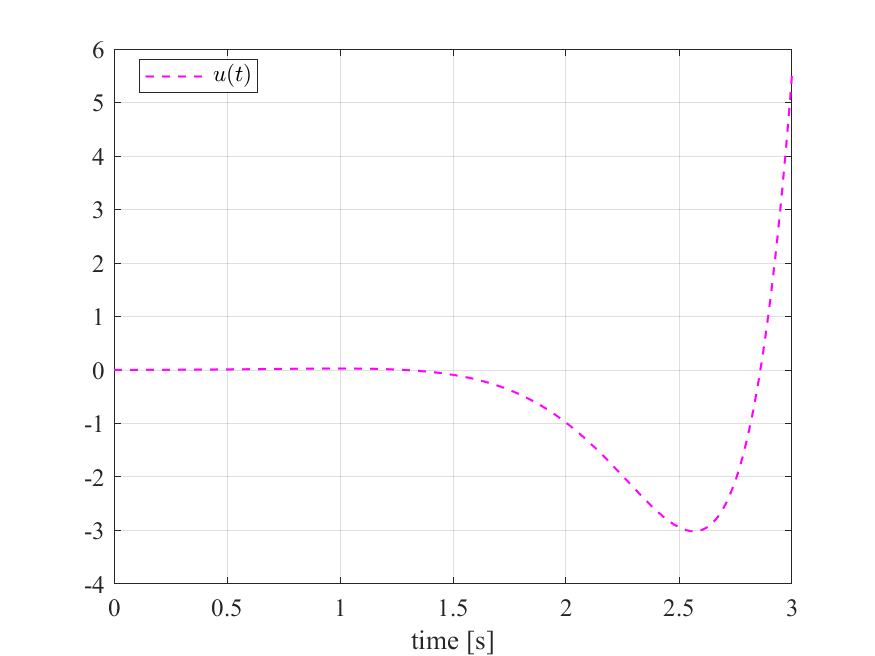
\includegraphics[width=1.0\textwidth]{control2.png}
    \caption{Управляющий сигнал}
\end{figure}

Вектор состояний системы будет выглядеть следующим образом:
\begin{figure}[ht]
  \centering
  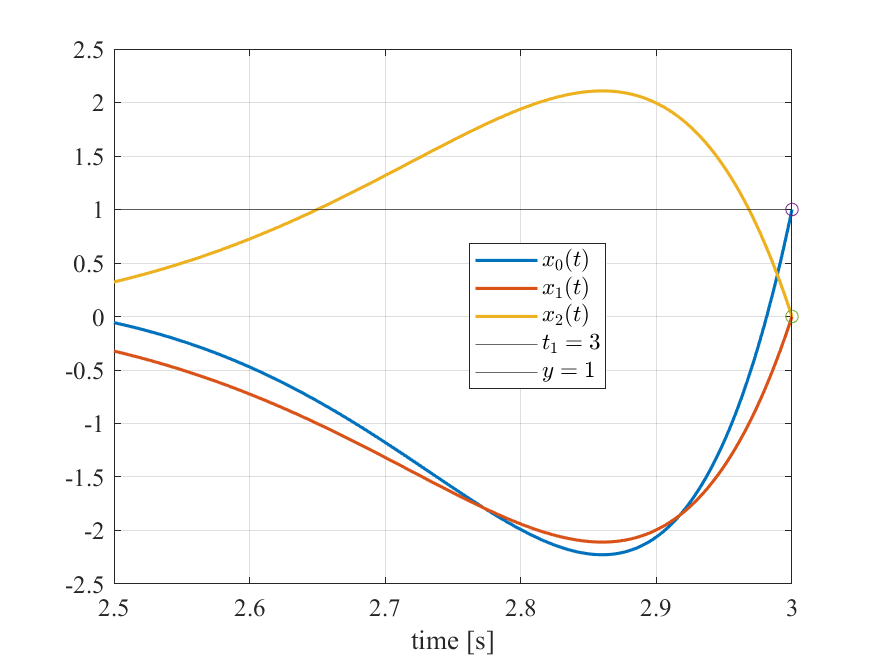
\includegraphics[width=1.0\textwidth]{controlability2.png}
  \caption{Состояния системы}
\end{figure}

\newpage
\subsection{Вывод}
Были рассмотрены две точки $x_1', x_1''$ и проверена их принадлежность управляемому
подпространству. Первая точка - принадлежит, вторая - нет.

Исследование системы в этом задании показало, что она не является полностью управляемой. 
Это было показано с помощью критерия Калмана, через управляемость собственных значений и жорданову форму системы.
При этом оказалось, что собственное число $\lambda_3=-1$ не является управляемым. 
Также был найден грамиан управляемости и проверены его собственные числа. 
Было получено, что одно из собственных чисел равно нулю, что говорит - система не является полностью управляемой.

Проведено моделирование системы с управлением, которое переводит систему в заданное состояние. 
Результаты показали, что  управление работает корректно.
\endinput